\section{Auswertung}
\label{sec:Auswertung}
\subsection{Brechnung der Fourier-Koeffizenten}
\subsubsection{Rechteckspannung}
  Für die Rechteckspannung ergibt sich mit der Gleichung \eqref{eqn:bn} und der Funktion \eqref{eqn:recht} die Fourier-Amplituden mit der Fuktion:
  \begin{equation}
    b_n = \frac{A}{n\pi}(1-cos(n\pi))
  \end{equation} .
  Die Werte sind in Tabelle \ref{fig:kr} dargestellt für $A =1$.
  \begin{table}
    \centering
    \caption{Fourier-Koeffizenten einer Rechteckspannung}
    \label{fig:kr}
    \sisetup{round-mode = places , round-precision = 2}
    \begin{tabular}{S[round-precision = 0] S}
      \toprule
       \text{Nr.} & \text{Fourier-Amplitude} \\
      \midrule
      1.000000000000000000e+00 & 6.366197723675813824e-01\\
      2.000000000000000000e+00 & 0.000000000000000000e+00\\
      3.000000000000000000e+00 & 2.122065907891937941e-01\\
      4.000000000000000000e+00 & 0.000000000000000000e+00\\
      5.000000000000000000e+00 & 1.273239544735162709e-01\\
      6.000000000000000000e+00 & 0.000000000000000000e+00\\
      7.000000000000000000e+00 & 9.094568176679733440e-02\\
      8.000000000000000000e+00 & 0.000000000000000000e+00\\
      9.000000000000000000e+00 & 7.073553026306460267e-02\\
      \bottomrule
      \end{tabular}
  \end{table}

\subsubsection{Sägezahnspannung}
Die Fourie-Koeffizenten der Sägezahnspannung lassen sich mit Zurhilfenahme der Gleichung \eqref{eqn:bn} und der Funktion \eqref{eqn:recht} durch folgende Gleichung brechnen:
\begin{equation}
  b_n = -\frac{A}{n\pi}
\end{equation}
Die Werte der Fourier-Koeffizenten finden sie in Tabelle \ref{fig:kd} dargestellt für $A = 1$.
\begin{table}
  \centering
  \caption{Fourier-Koeffizenten einer Sägezahnspannung}
  \label{fig:kd}
  \sisetup{round-mode = places , round-precision = 2}
  \begin{tabular}{S[round-precision = 0] S}
    \toprule
     \text{Nr.} & \text{Fourier-Amplitude} \\
    \midrule
    1.000000000000000000e+00 & -3.183098861837906912e-01\\
    2.000000000000000000e+00 & -1.591549430918953456e-01\\
    3.000000000000000000e+00 & -1.061032953945968971e-01\\
    4.000000000000000000e+00 & -7.957747154594767280e-02\\
    5.000000000000000000e+00 & -6.366197723675813547e-02\\
    6.000000000000000000e+00 & -5.305164769729844854e-02\\
    7.000000000000000000e+00 & -4.547284088339866720e-02\\
    8.000000000000000000e+00 & -3.978873577297383640e-02\\
    9.000000000000000000e+00 & -3.536776513153230134e-02\\
    \bottomrule
  \end{tabular}
\end{table}
\FloatBarrier
\subsubsection{Nadelimpuls}
  Die Fourier-Koeffizenten des Nadelimpuls werden mit Zurhilfenahme der Gleichung \eqref{eqn:an} und der Funktion \eqref{eqn:recht} durch die folgende Gleichung berechnet:
  \begin{equation}
    a_n = \frac{A}{n\pi} sin\left(\frac{n2\pi}{k}\right)
  \end{equation}
  Die Werte finden sie in Tabelle \ref{fig:kn} für verschiedene Werte von k dargestellt mit $A=1$.
\begin{table}
  \centering
  \caption{Fourier-Koeffizenten eines Nadelimpulses}
  \label{fig:kn}
  \begin{subfigure}{0.48\textwidth}
    \centering
  \label{fig:kn10}
  \sisetup{round-mode = places , round-precision = 2}
  \begin{tabular}{S[round-precision = 0] S}
    \toprule
     \text{Nr.} & \text{Fourier-Amplitude} \\
    \midrule
    1.000000000000000000e+00 & 1.870978567577278318e-01\\
    2.000000000000000000e+00 & 1.513653457281314008e-01\\
    3.000000000000000000e+00 & 1.009102304854209431e-01\\
    4.000000000000000000e+00 & 4.677446418943196488e-02\\
    5.000000000000000000e+00 & 7.796343665038751913e-18\\
    6.000000000000000000e+00 & -3.118297612628796386e-02\\
    7.000000000000000000e+00 & -4.324724163660896570e-02\\
    8.000000000000000000e+00 & -3.784133643203285713e-02\\
    9.000000000000000000e+00 & -2.078865075085865530e-02\\
    \bottomrule
  \end{tabular}
  \caption{mit $k = 10$}
\end{subfigure}
  \begin{subfigure}{0.48\textwidth}
    \centering
  \label{fig:kn100}
  \sisetup{round-mode = places , round-precision = 2}
  \begin{tabular}{S[round-precision = 0] S}
    \toprule
     \text{Nr.} & \text{Fourier-Amplitude} \\
    \midrule
    1.000000000000000000e+00 & 1.998684312479682632e-02\\
    2.000000000000000000e+00 & 1.994740365545007166e-02\\
    3.000000000000000000e+00 & 1.988177497291702608e-02\\
    4.000000000000000000e+00 & 1.979011241962616921e-02\\
    5.000000000000000000e+00 & 1.967263286166931816e-02\\
    6.000000000000000000e+00 & 1.952961407775311367e-02\\
    7.000000000000000000e+00 & 1.936139397678475829e-02\\
    8.000000000000000000e+00 & 1.916836964649249950e-02\\
    9.000000000000000000e+00 & 1.895099623599886401e-02\\
    \bottomrule
  \end{tabular}
  \caption{mit $k = 100$}
\end{subfigure}
\end{table}
\FloatBarrier
Aus Tabelle \ref{fig:kn}\subref{fig:kn100} ist ersichtlich, dass sich für hohe Werte von k ein sog. Dirac-Kamm ergibt.
\subsection{Vergleich mit den experimentel erfassten Fourier-Koeffizenten}
\label{sec:3.2}
\subsubsection{Rechteckspannung}
In Abbildung \ref{fig:pr} sind die rechnerisch und experimentel ermittelten Fourier-Koeffizenten aufgetragen. Die experimentellen Größen wurden alle mit einem Fehler
von 3\% versehen, da sie von einem Oszilloskop abgelesen wurden. Die Amplitude A der brechnetnen Werte wurde hier mit 10 Volt angenährt.
Dennoch ist zu beobachten, dass die Erwartungswerte nicht innerhalb der Fehlertoleranz liegen.
\begin{figure}
  \centering
  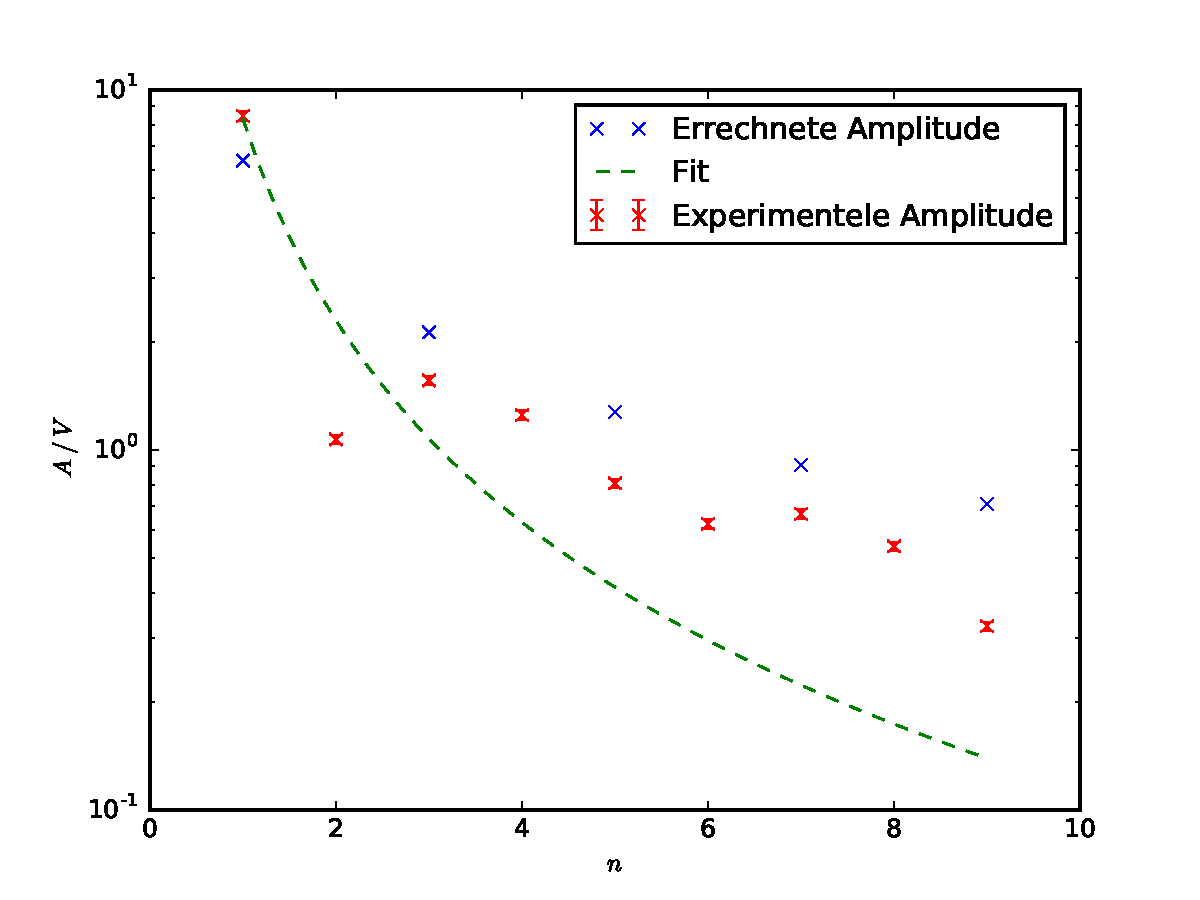
\includegraphics[width= \textwidth]{Plots/Rechteckplot.pdf}
  \caption{Rechnerische und experimentelle Fourier-Amplituden der Rechteckspannung}
  \label{fig:pr}
\end{figure}
\FloatBarrier
Der Fit wurde mit der Funktion \eqref{eqn:fit} druchgeführt. Hier liegt a bei $ 8, 3 \pm 0,6$
und b bei $1,86 \pm 0,27 $
\begin{equation}
  f(n , a , b) = a\frac{1}{n^b}
\label{eqn:fit}
\end{equation}
\subsubsection{Sägezahnspannung}
Auch hier wurden die rechnerisch und experimentel ermittelten Fourier-Koeffizenten in
ein Diagramm eingetragen (s.Abb.\ref{fig:dp}), wieder wurden
die experimentellen Größen mit einem Fehler von 3\% versehen und die Amplitude A mit 10 Volt
angenommen.
Zudem wurden die Erwartungswerte mit anderem Vorzeichen eingezeichnet, damit sich die
 Kurve den experimentellen Werten angleicht.
Werden nur die Erwatungswerte mit anderem Vorzeichen und die experimentellen Werte verglichen
 ist zu sehen, dass hier die Werte nur am Anfang der Messreihe außerhalb der Fehlertoleranz liegen.
\begin{figure}
  \centering
  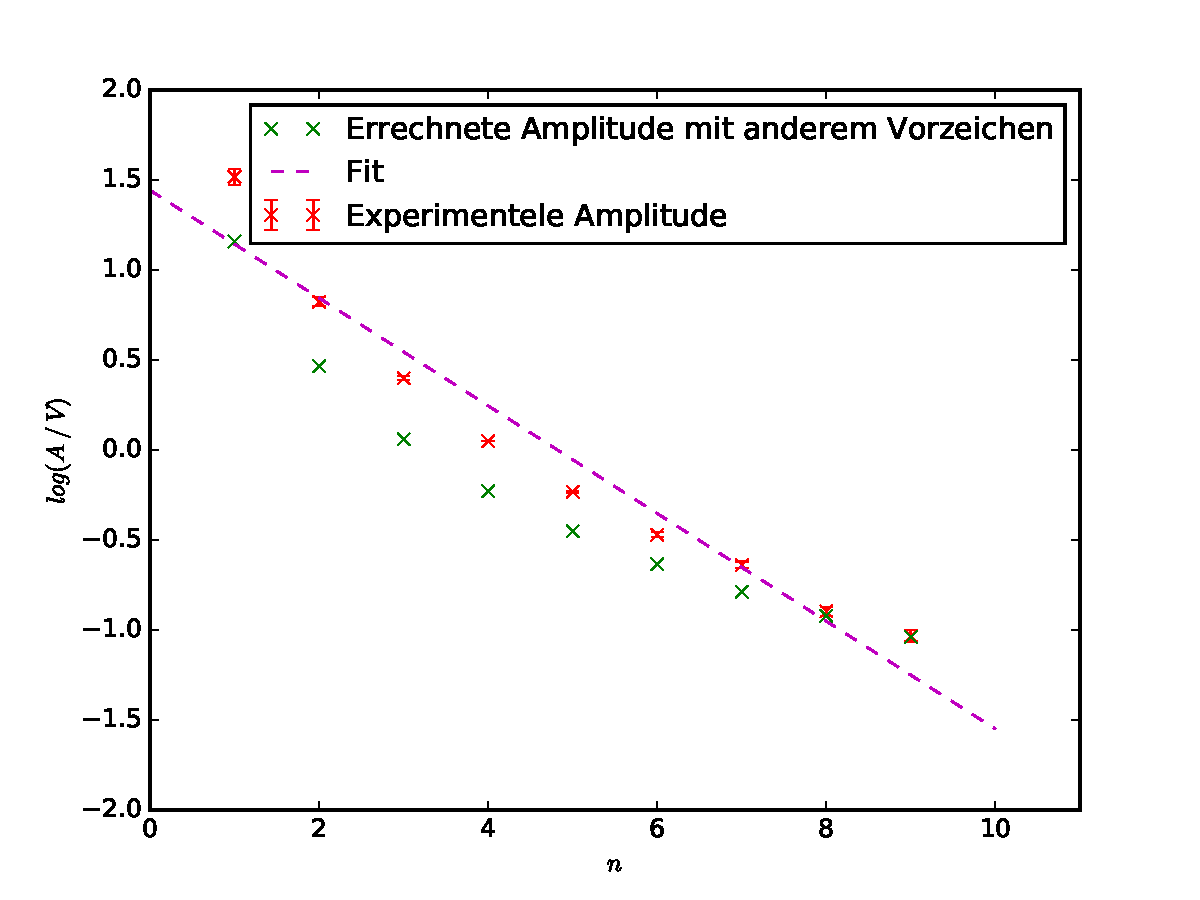
\includegraphics[width= \textwidth]{Plots/Dreieckplot.pdf}
  \caption{Rechnerische und experimentelle Fourier-Amplituden der Sägezahnspannung}
  \label{fig:dp}
\end{figure}
\FloatBarrier
Auch hier wurde der Fit mit der Formel \eqref{eqn:fit} durchgeführt mit den Werten
$a = 4,6 \pm 0,07 $ und $ b = 1,075 \pm 0,023 $.
\subsubsection{Nadelimpuls}
Wie auch in den beiden Messreihen davor sind auch hier rechnerisch und experimentel
ermittelte Fourier-Koeffizenten in Abbildung \ref{fig:np} eingezeichnet. Die experimentellen
Größen wurden wieder mit einem Fehler von 3\% versehen. Die Amplitude der rechnerischen Werte
für $ k = 10$ wurden wieder mit 10 Volt angenommen. Aber wie zu sehen ist passen die errechneten
Werte für $k = 10$ nicht zu unseren experimentellen Werten. Die Ampltitude A wurde für $k = 100$
mit 50 Volt angenommen. Hier sieht man sehr gut den sog. Dirac-Kamm der wiederum zu unseren
experimentellen Werten passt.
\begin{figure}
  \centering
  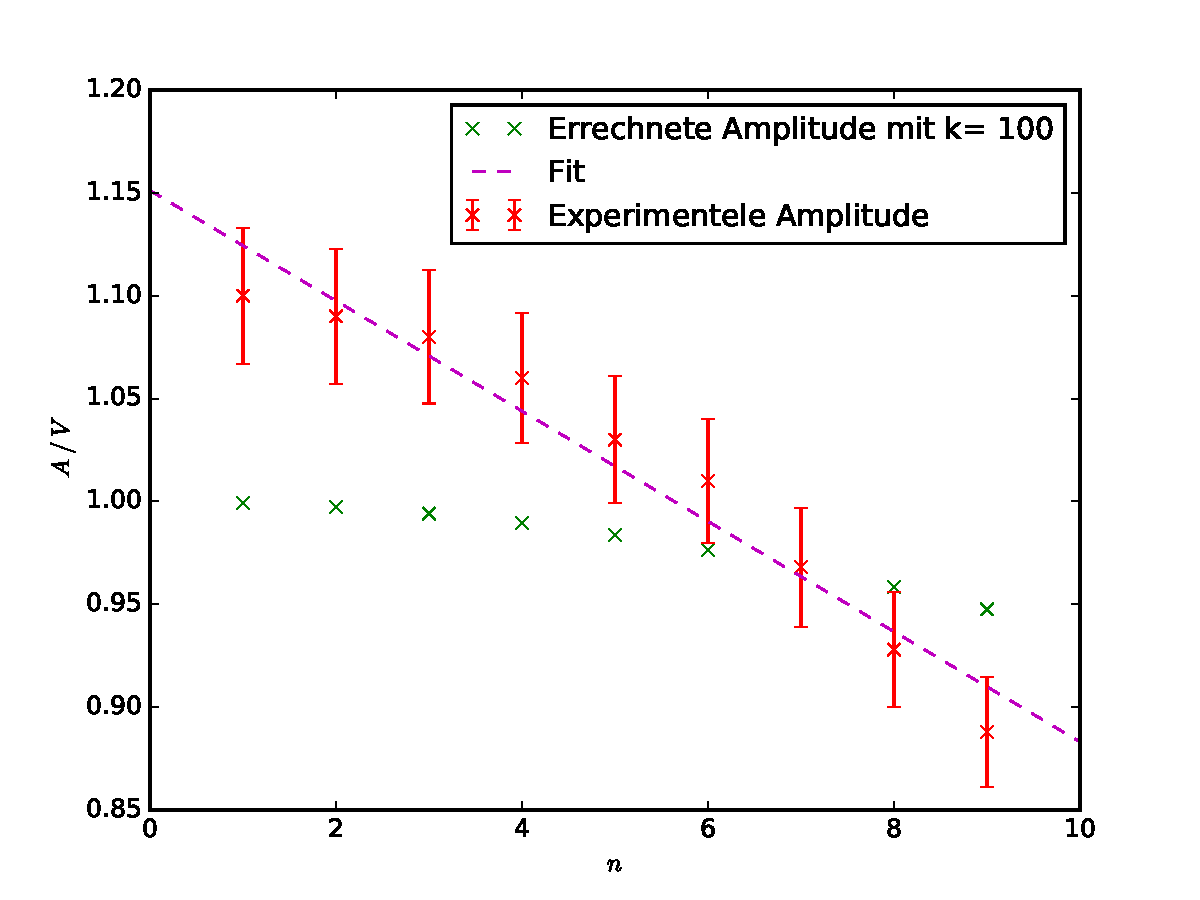
\includegraphics[width= \textwidth]{Plots/Nadelimpulsplot.pdf}
  \caption{Rechnerische und experimentelle Fourier-Amplituden des Nadelimpulses}
  \label{fig:np}
\end{figure}
\FloatBarrier
Der Fit hat die Werte $ a = 1,146 \pm 0,033 $ und $ b = 0,085 \pm 0,019$ mit Formel \eqref{eqn:fit}.

\subsection{Zusammensetzung der Schwingunsformen aus ihren Komponenten}
\label{sec:3.3}
\subsubsection{Reckteckspannung}
In der Abbildung \ref{fig:sr} ist eine Rechteckspannung zu sehen, die wir mit
unseren Fourier-Koeffizienten synthetisiert haben. Dafür das hier nur neun Oberschwingungen
addiert wurden kann man die approximierte Rechteckspannung gut erkennen.
\begin{figure}
  \centering
  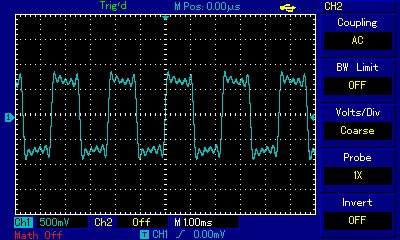
\includegraphics[height=7cm]{Prints/10.jpg}
  \caption{Sythetisierte Rechteckspannung in der neunten Oberschwingung}
  \label{fig:sr}
\end{figure}
\FloatBarrier
\subsubsection{Sägezahnspannung}
In der Abbildung \ref{fig:sd} ist eine synthetisierte Sägezahnspannung zu sehen. Auch hier
wurden wieder neun Oberschingungen summiert. Die Sägezahnspannung ist gut zu erkennen.
\begin{figure}
  \centering
  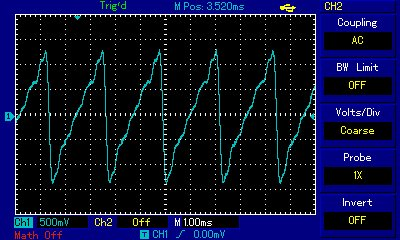
\includegraphics[height=7cm]{Prints/12.jpg}
  \caption{Sythetisierte Sägezahspannung in der neunten Oberschwingung}
  \label{fig:sd}
\end{figure}
\FloatBarrier
\subsubsection{Nadelimpuls}
In der folgenden Abbildung \ref{fig:sn} ist ein synthetisierter Nadelimpuls zu sehen. Wie bei
den vorherigen Synthesen ist auch hier die Summe aller neun Oberschingungen zu sehen. Auffällig
 ist, dass es hier Nulldurchgänge gibt die es eigentlich nicht geben sollte.
\begin{figure}
  \centering
  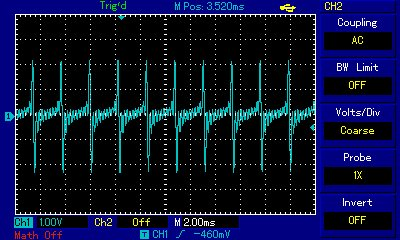
\includegraphics[height = 7cm]{Prints/14.jpg}
  \caption{Sythetisierte Nadelimpuls in der neunten Oberschwingung}
  \label{fig:sn}
\end{figure}
\FloatBarrier
